\documentclass[12pt,a4paper]{article}

% load packages
\usepackage{xcolor}
\usepackage{graphicx}
\usepackage{amsmath}
\usepackage{amsfonts}
\usepackage{amssymb}
\usepackage{listings}
\usepackage{hyperref}
\usepackage{algorithm}
\usepackage{algpseudocode}
\usepackage{float}
\usepackage{tabularx}
\usepackage{multirow}
\usepackage{booktabs}
\usepackage{setspace}
\setstretch{1.25}
\usepackage{appendix}
\usepackage[left=2cm,right=2cm,top=2cm,bottom=2cm]{geometry}

% set code style
\definecolor{codegreen}{rgb}{0,0.6,0}
\definecolor{codegray}{rgb}{0.5,0.5,0.5}
\definecolor{codepurple}{rgb}{0.58,0,0.82}
\definecolor{backcolour}{rgb}{0.95,0.95,0.92}


\title{Project 4 Report for Probelm 4.1}
\author{Zhu Liang}
\date{\today}

\begin{document}

\maketitle

\section{Project Description}
The primary objective of this project is the implementation of the parallel Strassen algorithm for matrix multiplication across three levels (1, 2, and 3), focusing on minimizing memory usage and communication costs.

Our approach utilizes a hierarchical multi master-slave tree (or leader-worker tree) structure. 
Each layer comprises a single leader and seven workers, where workers can serve as leaders for the subsequent layer, 
 facilitating the next level of the Strassen algorithm. 
This design allows the leader to distribute specific submatrices to its workers, 
 who later return their computed results. 
By limiting data exchange to only essential information between leaders and workers, 
 our implementation effectively reduces communication overhead and optimizes memory consumption.


\section{Algorithm Description}
The general idea of the parallel Strassen algorithm is to divide-and-conquer the matrix multiplication problem into subproblems. 
The subproblems are then distributed to different processors to compute.
The results are then collected and combined to form the final result.
This process can be repeated recursively until the 

\begin{algorithm}[htbp]
    \caption{Strassen Multiply Parallel}
    \label{alg:strassen_multiply_parallel}
    \begin{algorithmic}[1]
    \Procedure{StrassenMultiplyParallel}{$A, B, N, max\_level$}

        \For{$level \gets 1$ \textbf{to} $max\_level$}
            \State \Call{DistributeData}{$level$}  
        \EndFor
        
        \State $C \gets$ \Call{MatrixMultiply}{$A, B$}
        
        \For{$level \gets max\_level$ \textbf{down to} $1$}
            \State \Call{CollectResults}{$level$}
        \EndFor
        
        \State \Return $C$ on \textit{ROOT}
    \EndProcedure
    \end{algorithmic}
\end{algorithm}




This description is intentionally streamlined, 
omitting many details and supporting functions for brevity. 
More details can be gleaned from the source code file \texttt{functions.c}.

\section{Results}
\subsection{Performance}
Notice that the level 1, 2, 3 of the parallel Strassen algorithm requires 7, 49, 343 processors respectively to 
fully utilize the parallelism. We will run the parallel Strassen algorithm with 7, 49, 343 processors respectively.
\begin{table}[ht]
    \centering
    \begin{tabular}{cccc}
        \toprule
        & \multicolumn{3}{c}{Parallel Strassen Algorithm} \\
        \cmidrule(lr){2-4}
        (in seconds) &  level 1  &  level 2  &  level 3 \\
        & (cores = 7) & (cores = 49) & (cores = 343) \\
        \midrule
        \( N = 2^8 \)  & 0.029430 & 0.010317 & 0.040137 \\
        \( N = 2^{10} \) & 1.757423 & 0.284435 & 0.274502 \\
        \( N = 2^{12} \) & 63.811983 & 9.049598 & 2.902417 \\
        \bottomrule
    \end{tabular}
    \caption{Performance of the Parallel Strassen Algorithm at different levels.}
    \label{tab:results}
\end{table}


\subsection{Speedup}
Speedup is a metric that quantifies the performance improvement of a parallel algorithm compared to its sequential counterpart. 
The orginal speedup \( S \) for \( P \) processors for size $N$ problem is defined as:

\begin{equation*}
    S(P, N) = \frac{T(1,N)}{T(P, N)}
\end{equation*}

where \( T(1,N) \) is the execution time of the sequential algorithm and 
 \( T(P, N) \) is the execution time of the parallel algorithm using \( P \) processors.

However, in our case, the sequential algorithm on single core is not implemented. Instead, 
 we use the performance of the parallel algorithm with \( P = 7 \) as the baseline.
The updated speedup \( S \) is defined as:

\begin{equation}
    \label{eqn:updated_speedup}
    S(P, N) = 7 \times \frac{T(7,N)}{T(P, N)}
\end{equation}


 Using the data from Table \ref{tab:results}, 
  we can compute the speedup for matrix multiplication for different 
  matrix sizes \( N \) and varying number of processors \( P \). 
The speedup values for each \( N \) (under level 2 and level 3) are plotted in the following Figure \ref{fig:speedup_curve}.

\begin{figure}
    \centering
    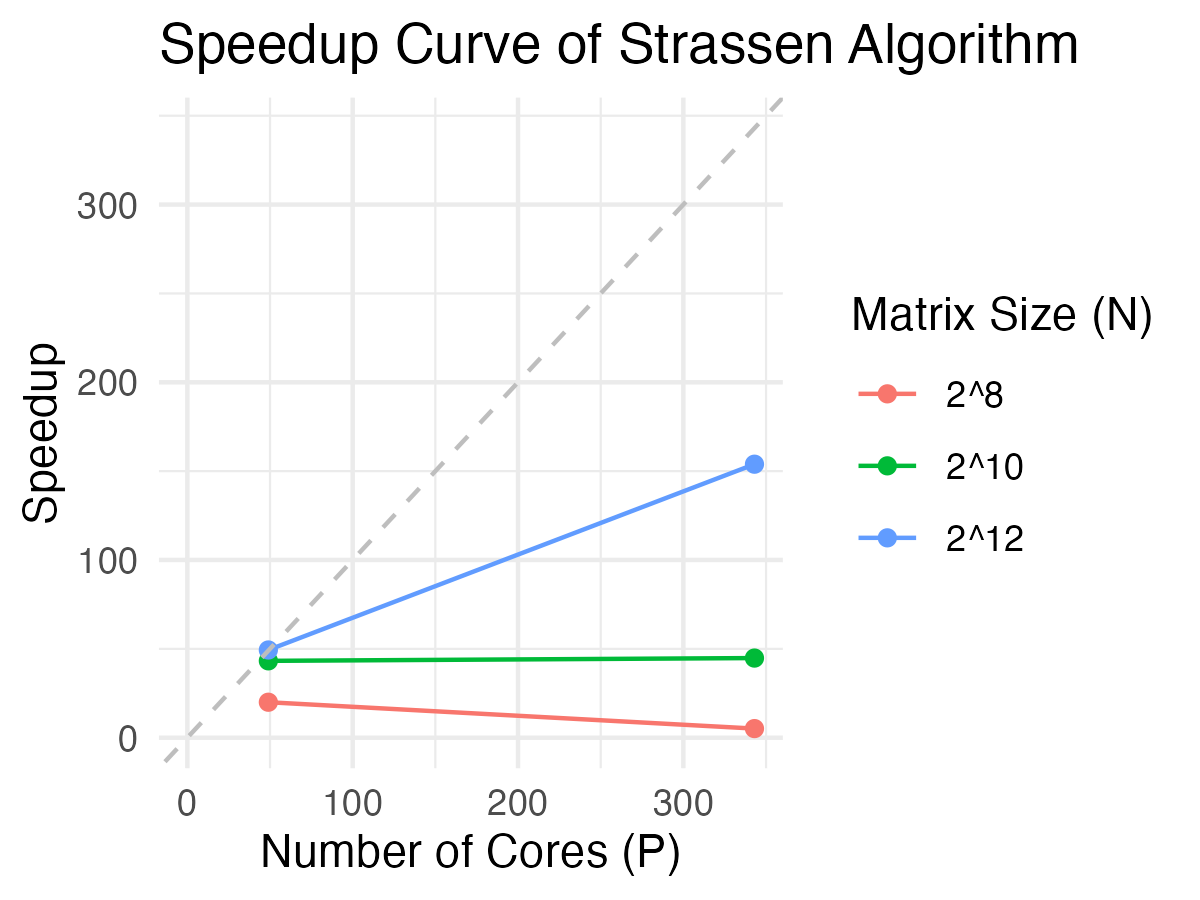
\includegraphics[width=0.6\textwidth]{speedup_curve.png}
    \caption{Speedup Curve for Matrix Sizes \( N \)}
    \label{fig:speedup_curve}
\end{figure}
    


\section{Analysis}


\appendix
\label{app:myappendix}

\section*{File Notes}
The source code of the program is in the \texttt{project4} folder. 
For more details, please refer to the \texttt{README.md} file in the folder.

\end{document}


